\documentclass[fontsize=24pt]{beamer}

% Language and encoding
\usepackage[english]{babel}
\usepackage[utf8]{inputenc}

% Bibliography and citation
%\usepackage[backend=biber]{biblatex}

% Colors
\usepackage{xcolor}
\selectcolormodel{cmyk}

% New colors
\definecolor{grey}{rgb}{0.5,0.5,0.5}
\definecolor{darkgrey}{rgb}{0.25,0.25,0.25}
\definecolor{brightgrey}{rgb}{0.75,0.75,0.75}
\definecolor{water}{rgb}{0.5,0.7,1}
\definecolor{solution}{rgb}{.3,.4,0}
\definecolor{sphere}{rgb}{.1,.1,.1}
\definecolor{substrate}{rgb}{.75,.75,.75}
\definecolor{gold}{rgb}{1,.8,0}
\definecolor{vacuum}{rgb}{.7,.5,.8}
\definecolor{angle}{rgb}{0,0,1}
\definecolor{omega}{rgb}{0,0,0}
\definecolor{spy}{rgb}{.9,0,0}
\definecolor{crosssection}{rgb}{0,1,0}
\definecolor{goldray}{rgb}{.8,.6,0}
\definecolor{split}{rgb}{1,0,0}

% Images
%\usepackage[font=normalsize]{caption}
\usepackage[font=normalsize]{subcaption}
\usepackage{caption}
%\usepackage{subcaption}
\usepackage{placeins}
\usepackage{wrapfig}
\usepackage{tikz}
\usepackage{pgfplots}
\usepackage{adjustbox}
\usepackage{changepage}
%\usepackage{environ}
\usetikzlibrary{arrows, calc, decorations.markings}

% Configure tikz
\tikzset{
%    x=0.1\textwidth,
%    y=0.1\textwidth,
    font={\fontsize{24pt}{30}\selectfont},
    }

% Extracts coordinate
\newdimen\XCoord
\newdimen\YCoord
\newcommand*{\ExtractCoordinate}[1]{\path (#1); \pgfgetlastxy{\XCoord}{\YCoord};}

% Configure captions
\renewcommand\thesubfigure{\arabic{subfigure}}

% Physics and maths
\usepackage{physics}
\usepackage{amsmath}
\usepackage{mathtools}
\usepackage{upgreek}
\usepackage{amssymb}
\usepackage[separate-uncertainty=true,
            list-units = single,
            list-separator = {;\,},
            exponent-product=\cdot,
            ]{siunitx}

% Poster specific
\usepackage[orientation=portrait,
            size=a0,
            scale=1.0,
            ]{beamerposter}
\usepackage[absolute,
            overlay,
            ]{textpos}
\setlength{\TPHorizModule}{1cm}
\setlength{\TPVertModule}{1cm}
\usetheme{Dreuw}

%bibliography
\bibliographystyle{plain}

% Title
\graphicspath{{../figures/}}
\title[Metamaterials]{Metamaterials}
\author[Sattler \& Marquardt]{Alexander Sattler \\ \& Michael Marquardt}
\institute[Universität Stuttgart]{Universität Stuttgart}
\date{18.06.2018}

% New commands for posters
\usepackage{varwidth}
\newcommand\Umbruch[2][0.15\linewidth]{
    \begin{varwidth}{#1}
        \flushleft #2   
    \end{varwidth}}
    \newenvironment{indentitemize}{%
        \begin{itemize}%
            \addtolength{\itemindent}{2ex}%
            \setlength{\leftmargin}{2ex}%
            \setlength{\topsep}{0pt}%
        }
        {%
        \end{itemize}%
    }

\newcommand*\circled[1]{\tikz[baseline=(char.base)]{\node[shape=circle,draw,inner sep=.4ex, line width = 1.5mm] (char) {#1};}}

\begin{document}

% Example using columns
\begin{frame}{}
\begin{columns}[t]

\begin{column}{0.48\linewidth}
    \begin{block}{\circled{1} Introduction}
        \textbf{Aim:}
\begin{itemize}
\item{Fabrication of split-ring resonators (SRRs) by using shadow nanosphere lithography}
\item{Analysing the spectral properties of the SRRs with FTIR}
\end{itemize}
\textbf{Motivation:}
\begin{itemize}
\item{Fast, cheap and large area fabrication technique}
\item{Tunable optical metamaterials resonance in the range of \SI{100}{THz}}
\end{itemize}

    \end{block}
    
     \begin{block}{\circled{2} Theory}
        Metamaterials are materials with a structure which is smaller then the wavelenght of ligth. The special properties of metamaterials is  based on the fact that they have a negative permeability $\mu$ and permittivity $\epsilon$. That leads to a negative refractive index $n = \sqrt{\epsilon \cdot \mu}$. 
The Lorentz-Oscillator model describes the optical characteristics of intraband  and the Drude model of the interband transitions and both can show  a negative $\epsilon$. The negative $\mu$ can be explained with the Kirchhoff's circuit laws. \\
The reflection spectrum of SRR shows frequency and polarisation dependencies \ref{spectrum_theory}.
\begin{figure}[H]
\centering
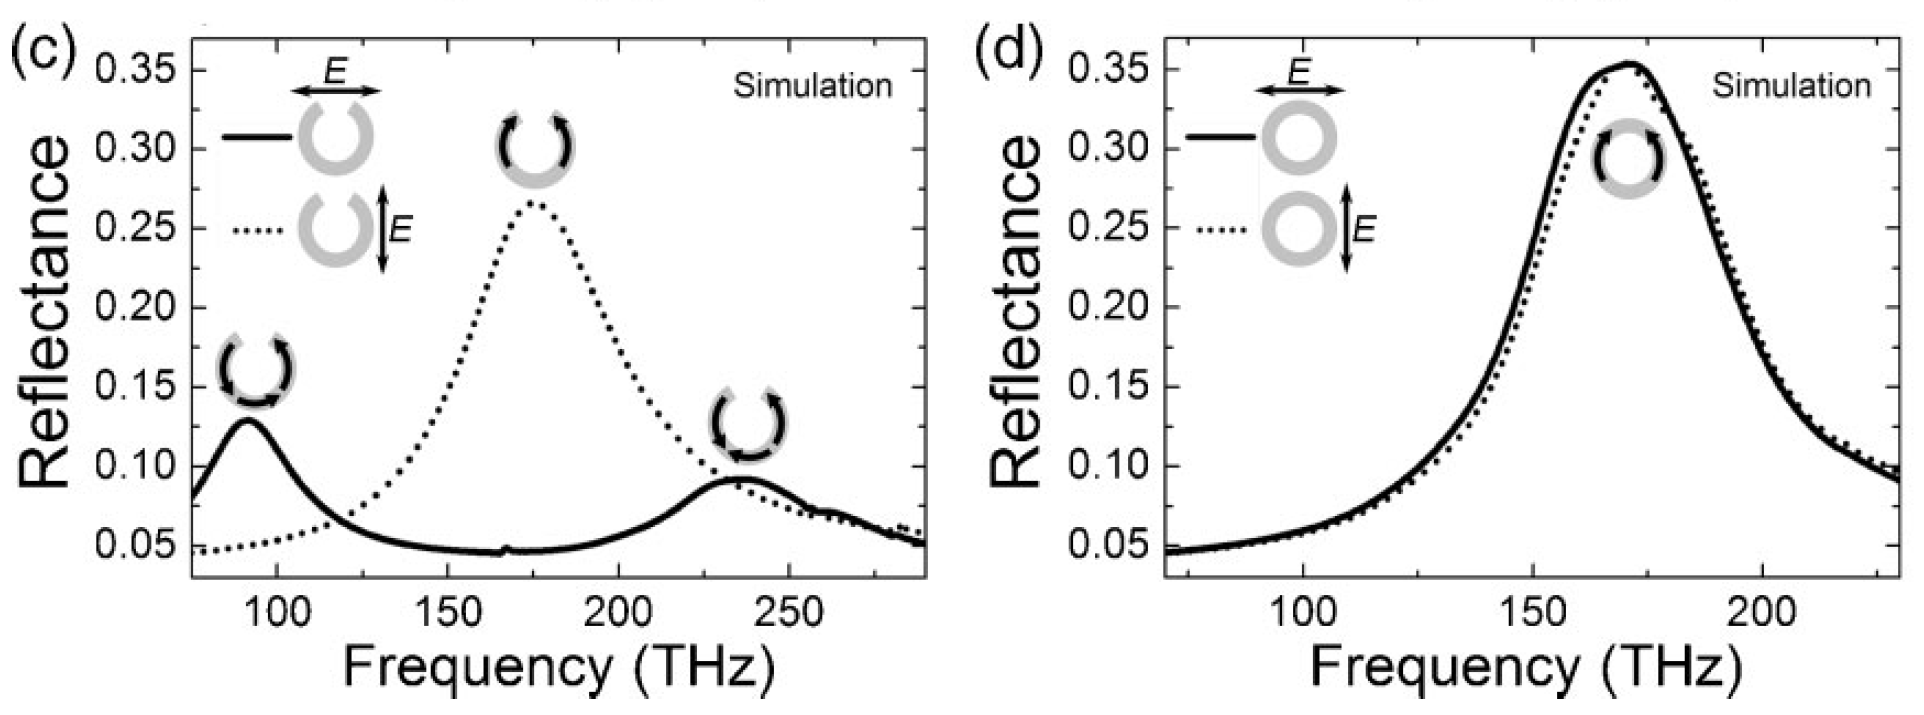
\includegraphics[scale=1]{../figures/spectrum_theory.png}
\caption{Simulated reflection spectrum of SRR and a full ring for different polarisations. \cite{paper_Giessen_meta}  }
    \label{spectrum_theory}
\end{figure}

    \end{block}    

    \begin{block}{\circled{3} Evaporation}
        \begin{figure}[htbp]
\begin{subfigure}[t][][t]{0.72\textwidth}
    \begin{tikzpicture}
    [x=0.06667\textwidth, y=0.06667\textwidth]
    \draw (0,0) rectangle (15,7);
    % chamber
    \draw[fill=vacuum]
        (.5,1.5) rectangle (3.5,6.5);
    \draw[fill=gold]
        (1.7,1.95)--
        (2.3,1.95)--
        (2.3,1.8)--
        (1.7,1.8)--
        (1.7,1.95);
    \draw[fill=darkgrey]
        (1,2.1)--
        (1.65,2.1)--
        (1.75,1.8)--
        (2.25,1.8)--
        (2.35,2.1)--
        (3,2.1)--
        (3,2)--
        (2.4,2)--
        (2.3,1.7)--
        (1.7,1.7)--
        (1.6,2)--
        (1,2)--
        (1,2.1);
    \draw[gold,dashed,line width=0.003\textwidth]
        (2,2) -- (2,5);
    \coordinate (a) at (2,5);
    \def\thetheta{20}
    \draw[fill=darkgrey,rotate=\thetheta,shift={(a)}]
        (-1,-.1) rectangle (1,.1);
    \draw[angle,dotted,line width=0.003\textwidth,rotate=\thetheta,shift={(a)}]
        (0,-.1) -- (0,-1.8);
    \draw[angle,line width=0.002\textwidth,shift={(a)}]
        (0,-1.5) arc(270:270+\thetheta:1.5);
    \draw[fill=substrate,rotate=\thetheta,shift={(a)}]
        (-.2,-.1) rectangle (.2,.-.2)
        (-.8,-.1) rectangle (-.4,.-.2)
        (.4,-.1) rectangle (.8,.-.2);
    \draw[fill=sphere,rotate=\thetheta,shift={(a)}]
        (-.2,-.2) rectangle (.2,.-.22)
        (-.8,-.2) rectangle (-.4,.-.22)
        (.4,-.2) rectangle (.8,.-.22);
    \draw[omega,line width=0.01\textwidth,rotate=\thetheta,shift={(a)}]
        (0,.1) -- (0,1.2);
    \draw[omega,<->,line width=0.003\textwidth,rotate=\thetheta,shift={(a)}]
        (0,.4)++(120:.5) arc(120:420:.5 and .15);
    % zoom
    \coordinate (sp1) at ($(a)+(\thetheta:.6)+.16*(sin{\thetheta},-cos{\thetheta})$);
    \coordinate (sp2) at (5.5,3.85);
    \draw[spy,line width=0.002\textwidth]
        (sp1) circle(.25)
        (sp2) circle(1.9)
        ($(sp1)+(90:.25)$)--($(sp2)+(100:1.9)$)
        ($(sp1)+(230:.25)$)--($(sp2)+(220:1.9)$);
    \coordinate (s) at (4,1);
    \draw[fill=substrate,shift={(s)}]
        (0.5,4.1) rectangle (2.5,4.3)
        (0.5,1.5) rectangle (2.5,3.5);
    \foreach \i in {1.63,1.9764,...,3.41}
        \foreach \j in {0.6,0.8,...,2.41}
            \filldraw[sphere,shift={(s)}] (\j,\i) circle (0.105);
    \foreach \i in {1.8032,2.1496,...,3.41}
        \foreach \j in {0.7,0.9,...,2.41}
            \filldraw[sphere,shift={(s)}] (\j,\i) circle (0.105);
    \foreach \i in {0.6,0.8,...,2.41}
        \filldraw[sphere,shift={(s)}]
            (\i,4.01) ellipse [x radius=0.105,y radius=0.09];
    % second zoom
    \coordinate (sp3) at (6.1,2.9);
    \coordinate (sp4) at (7.7,1.3);
    \draw[spy,line width=0.002\textwidth]
        (sp3) circle(.25)
        (sp4) circle(1.2)
        ($(sp3)+(60:.25)$)--($(sp4)+(70:1.2)$)
        ($(sp3)+(210:.25)$)--($(sp4)+(194:1.2)$);
    \filldraw[sphere,shift={($(sp4)-(0,0.148)$)}]
        (-.5,0.433) circle(.525)
        (.5,0.433) circle(.525)
        (0,-0.433) circle(.525);
    % cross section
    \coordinate (m) at (12,2.5);
    \def\shift{1.2}
    \coordinate (lda) at
        ($
        (m)
        +(-\shift,0.6)
        +(cos{\thetheta},0)
        -(1/cos{\thetheta}*sin{\thetheta},0)
        +(sin{\thetheta}*sin{\thetheta}/cos{\thetheta},0)
        $);
    \coordinate (ldb) at
        ($
        (m)
        +(-\shift,3.5)
        +(cos{\thetheta},0)
        +(2.9/cos{\thetheta}*sin{\thetheta},0)
        -(1/cos{\thetheta}*sin{\thetheta},0)
        +(sin{\thetheta}*sin{\thetheta}/cos{\thetheta},0)
        $);
    \coordinate (rua) at
        ($
        (m)
        +(+\shift,0.6)
        -(cos{\thetheta},0)
        -(1/cos{\thetheta}*sin{\thetheta},0)
        -(sin{\thetheta}*sin{\thetheta}/cos{\thetheta},0)
        $);
    \coordinate (rub) at
        ($
        (m)
        +(+\shift,3.5)
        -(cos{\thetheta},0)
        +(2.9/cos{\thetheta}*sin{\thetheta},0)
        -(1/cos{\thetheta}*sin{\thetheta},0)
        -(sin{\thetheta}*sin{\thetheta}/cos{\thetheta},0)
        $);
    \draw[goldray,fill=gold,fill opacity=0.3,line width=0.003\textwidth]
        (lda)--(ldb)--
        (rub)--(rua)--
        (lda);
    \filldraw[gold]
        (lda)rectangle($(rua)+(0,0.08)$);
    \coordinate (rda) at
        ($
        (m)
        +(\shift,0.6)
        -(cos{\thetheta},0)
        +(1/cos{\thetheta}*sin{\thetheta},0)
        -(sin{\thetheta}*sin{\thetheta}/cos{\thetheta},0)
        $);
    \coordinate (rdb) at
        ($
        (m)
        +(\shift,3.5)
        -(cos{\thetheta},0)
        -(2.9/cos{\thetheta}*sin{\thetheta},0)
        +(1/cos{\thetheta}*sin{\thetheta},0)
        -(sin{\thetheta}*sin{\thetheta}/cos{\thetheta},0)
        $);
    \coordinate (lua) at
        ($
        (m)
        +(-\shift,0.6)
        +(cos{\thetheta},0)
        +(1/cos{\thetheta}*sin{\thetheta},0)
        +(sin{\thetheta}*sin{\thetheta}/cos{\thetheta},0)
        $);
    \coordinate (lub) at
        ($
        (m)
        +(-\shift,3.5)
        +(cos{\thetheta},0)
        -(2.9/cos{\thetheta}*sin{\thetheta},0)
        +(1/cos{\thetheta}*sin{\thetheta},0)
        +(sin{\thetheta}*sin{\thetheta}/cos{\thetheta},0)
        $);
    \draw[goldray,fill=gold,opacity=0.8,fill opacity=0.1,dashed,line width=0.003\textwidth]
        (rda)--(rdb)--
        (lub)--(lua)--
        (rda);
    \filldraw[gold]
        (rda)rectangle($(lua)+(0,0.08)$);
    \draw[crosssection,dotted,line width=0.003\textwidth,shift={(sp4)}]
        (-1.2,0)--(1.2,0);
    \draw[crosssection,line width=0.003\textwidth,shift={(m)}]
        (-2.5,0)rectangle(2.5,3.5);
    \draw[crosssection,line width=0.002\textwidth]
        (sp4)++(1.2,0)--($(m)+(-2.5,2)$);
    \filldraw[sphere,shift={(m)}]
        (\shift,1.6) circle(1)
        (-\shift,1.6) circle(1);
    \draw[fill=substrate,shift={(m)}]
        (-2.3,0.2)rectangle(2.3,.6);
    \draw[omega,<->,line width=0.002\textwidth,shift={(m)}]
        (0,2.9)++(120:.55) arc(120:420:.55 and .1);
    \draw[angle,dashed,line width=0.003\textwidth,shift={(m)}]
        (0,0.6)--(0,3.5);
    \coordinate (rellda) at ($(m)-(lda)+(0,0.6)$);
    \ExtractCoordinate{rellda}
    \coordinate (point) at ($(m)+(0,\XCoord/sin{\thetheta}*cos{\thetheta})$);
    \draw[angle,line width=0.002\textwidth]
        ($(point)+(0,0.9)+(0,0.6)$) arc(90:90-\thetheta:0.9);
    % split-ring
    \coordinate (n) at ($(m)+(1.6,0)$);
    \draw[split,line width=0.002\textwidth,shift=(m)]
        (-0.8,0.4)rectangle(0.8,0.8)
        (0,0.4)--(1.6,-0.2);
    \draw[split,line width=0.002\textwidth,fill=substrate,shift=(n)]
        (-0.8,-0.2)rectangle(0.8,-1.8);
    \coordinate (O) at ($(n)-(0,1)$);
    \coordinate (split1) at (\XCoord,0);
    \coordinate (relrua) at ($(m)-(rua)+(0,0.6)$);
    \ExtractCoordinate{relrua}
    \coordinate (split) at ($(split1)+(0,\XCoord)$);
    \ExtractCoordinate{split}
    \draw[fill=gold]
        (O)++(-55:\XCoord)
        arc(-55:235:\XCoord)
        --($(O)+(235:\YCoord)$)
        arc(235:-55:\YCoord)
        --($(O)+(-55:\XCoord)$);
    % symbols
    \draw[omega] (2.6,6) node{$\omega$};
    \draw[angle] (2.2,3.8) node{$\theta$};
    \draw[omega] (11.2,5.7) node{$\omega$};
    \draw[angle] (12.12,5.1) node{$\theta$};
    \draw[decoration={
        markings,
        mark=at position 0 with {\arrow[scale=4,shift={(0.025,0)},black]{<}};,
        mark=at position 1 with {\arrow[scale=4,black]{>}};
    },postaction={decorate}] (1.1,2.3)--(1.1,4.5);
    \draw[] (1.1,3.4) node[above,rotate=90]{$\approx\SI{60}{\centi\metre}$};
    % text
    \draw[] (0.7,1.8)--(0.7,0.5) node[right]{vacuum chamber};
    \draw[] (2,1.9)--(2,1) node[right]{molten gold};
    \draw[] (2,2.5)--(3.8,1.5) node[right]{gold beam};
    \draw[] (1.9,5.3)--(4,6.5) node[right]{rotatable holder};
    \draw[] (2.6,5.05)--(4,6) node[right]{probe};
    \draw[] (6.4,5.2)--(7.2,5.5) node[right]{substrate};
    \draw[] (6.4,5)--(7.2,5) node[right]{mask};
    \draw[] (8.5,1.6)--(9,1) node[right]{sphere ($\varnothing\approx\SI{5}{\micro\metre}$)};
    \draw[] (7.7,1.3)--(9,0.5) node[right]{hole};
    \draw[] (13.6,1.9)--(12.5,1.9) node[left]{gold film};
    \draw[] (11.6,3.15)--(11.6,2.2);
    \draw[] (12.6,5.8)--(12.6,6.5) node[right]{gold beam};
    \draw[crosssection] (9.5,6.5) node[right]{cross section};
    \end{tikzpicture}
    \subcaption{Schematic drawing of the evaporation process.}
\end{subfigure}
\hfill
\begin{subfigure}[t][][t]{0.26\textwidth}
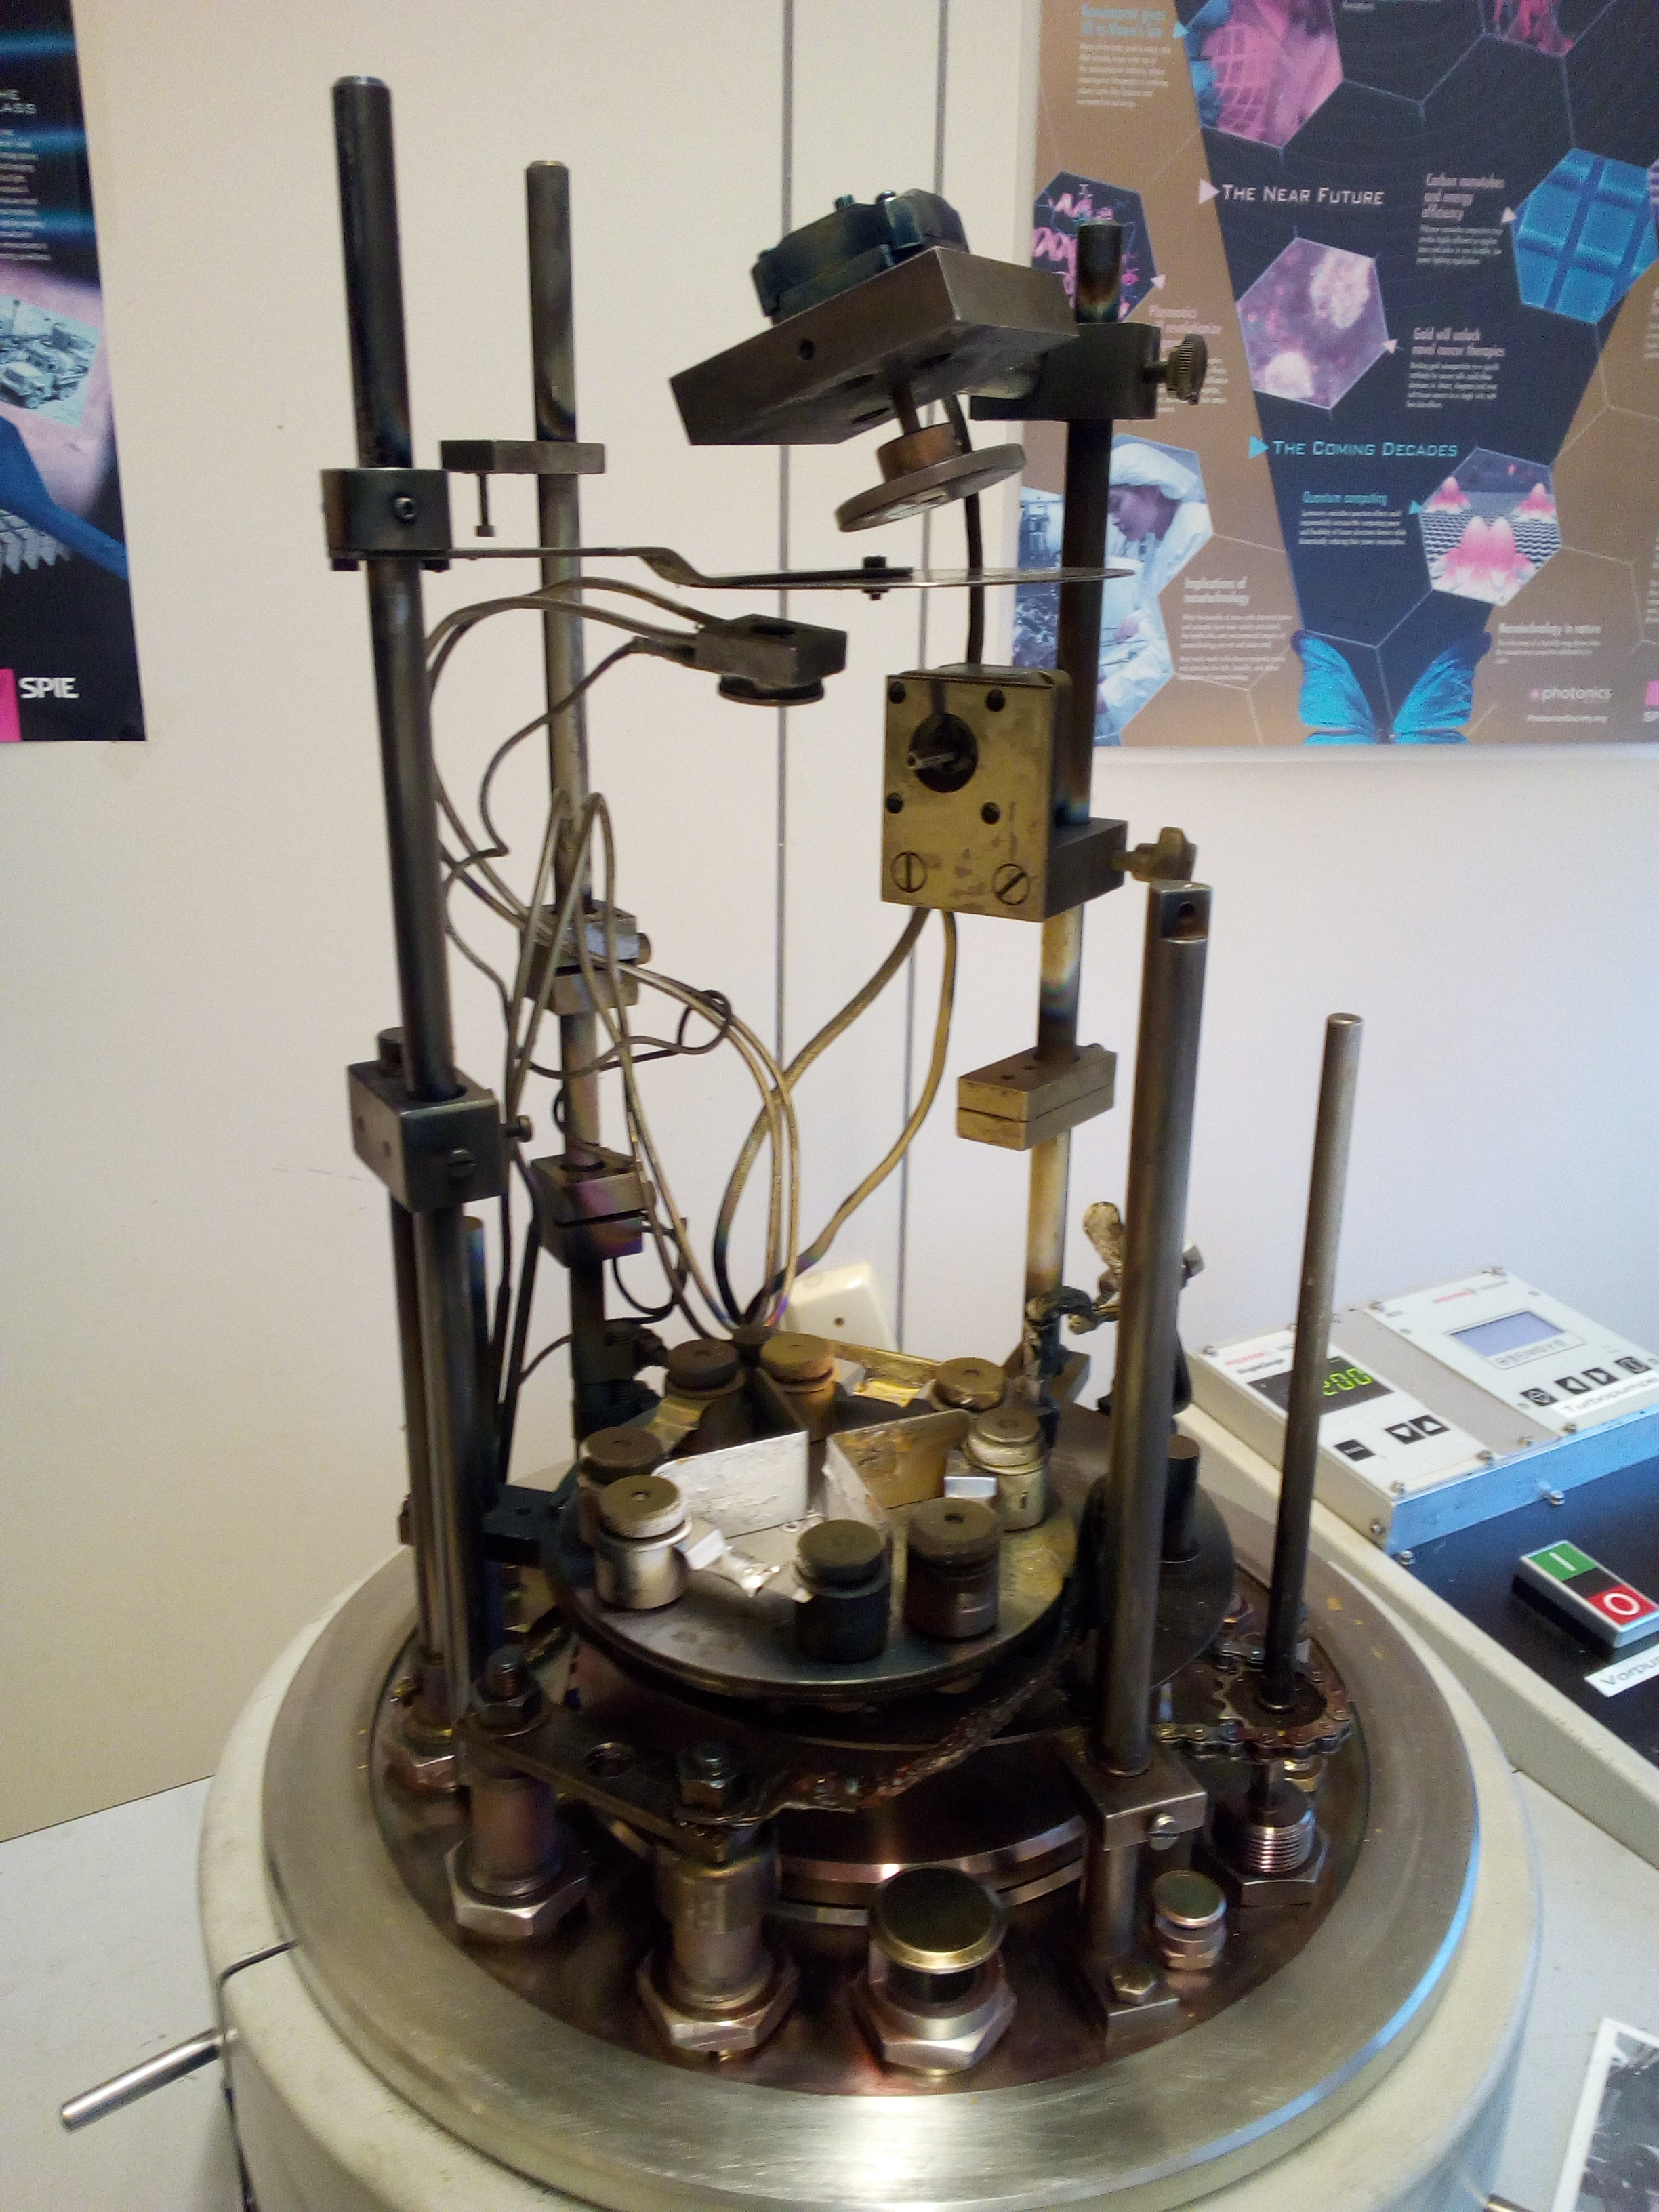
\includegraphics[width=0.97\textwidth]{chamber.jpg}
\subcaption{Evaporation chamber.}
\end{subfigure}
\end{figure}
    \end{block}

    \begin{block}{\circled{4} Fabrication of a Monolayer Mask}
        \begin{figure}[htbp]
\begin{subfigure}[t][][t]{0.48\textwidth}
    \begin{tikzpicture}
    [x=0.1\textwidth, y=0.1\textwidth]
    \draw (0,0) rectangle (10,5);
    \draw[thick] (0.5,4.5) circle(0.3) node{1};
    \filldraw[orange]
        (1,2.2) .. controls (0.8,2.5) ..
        (1.2,3.5) .. controls (1.6,2.5) ..
        (1.4,2.2);
    \filldraw[red]
        (1.2,3) .. controls (1.4,2.5) ..
        (1.2,2.3) .. controls (1,2.5) ..
        (1.2,3);
    \draw[fill=darkgrey]
        (0.2,0.2)--
        (2.2,0.2)--
        (1.4,1.2)--
        (1.4,2.2)--
        (1,2.2)--
        (1,1.2)--
        (0.2,0.2);
    \draw[fill=brightgrey]
        (1.2,3.5)--
        (0.4,3.2)--
        (0.38,3.25)--
        (1.2,3.6)--
        (1.6,3.63)--
        (1.8,3.7)--
        (5,3.7)--
        (5,3.4)--
        (1.8,3.4)--
        (1.6,3.47)--
        (1.2,3.5);
    \filldraw[red,scale=0.5,shift={(11.5,7)}]
        (0,.5)--
        (2,.5)--
        (2,1)--
        (3,0)--
        (2,-1)--
        (2,-.5)--
        (0,-.5);
%    \draw[fill=red]
%        (4,1)--
%        (6,1)--
%        (6,0.5)--
%        (7,1.5)--
%        (6,2.5)--
%        (6,2)--
%        (4,2)--
%        (4,1);
    \draw[fill=brightgrey,shift={(8.5,4.5)}]
        (0,0)--
        (0.025,0.05)--
        (0.525,-0.2)..controls(0.6,-0.25)..
        (0.525,-0.3)--
        (-0.175,-0.65)--
        (-0.16,-1)--
        (-0.11,-1.1)--
        (-0.11,-4)--
        (-0.365,-4)--
        (-0.365,-1.1)--
        (-0.315,-1)--
        (-0.3,-0.65)..controls(-0.25,-0.6)..
        (-0.2,-0.57)--
        (0.48,-0.25)--
        (0,0);
     % text
     \draw[] (1.5,0.5)--(2.5,0.5) node[right]{Bunsen burner};
     \draw[] (2.5,3.5)--(2.5,2.9) node[right]{glass pipette};
     \draw[] (8.45,4.5)--(8,4.5) node[left]{reduce the size of the opening};
    \end{tikzpicture}
    \subcaption{Bending of a glass pipette through melting.}
\end{subfigure}
\hfill
\begin{subfigure}[t][][t]{0.48\textwidth}
    \begin{tikzpicture}
    [x=0.1\textwidth, y=0.1\textwidth]
    \draw (0,0) rectangle (10,5);
    \draw[thick] (0.5,4.5) circle(0.3) node{2};
    \filldraw[water] (0.5,0.5) rectangle (9.5,2.2);
    \draw[fill=grey]
        (0.2,2.5)--
        (0.5,2.5)--
        (0.5,0.5)--
        (9.5,0.5)--
        (9.5,2.5)--
        (9.8,2.5)--
        (9.8,0.2)--
        (0.2,0.2)--
        (0.2,2.5);
    \draw[fill=solution,shift={(5,1.5)},rotate=250,scale=1.2]
        (0,0)--
        (0.025,0.05)--
        (0.525,-0.2)..controls(0.6,-0.25)..
        (0.525,-0.3)--
        (-0.175,-0.65)--
        (-0.16,-1)--
        (-0.11,-1.1)--
        (-0.11,-4)--
        (-0.365,-4)--
        (-0.365,-1.1)--
        (-0.315,-1)--
        (-0.3,-0.65)..controls(-0.25,-0.6)..
        (-0.2,-0.57)--
        (0.48,-0.25)--
        (0,0);
    \draw[fill=brightgrey,shift={(5,1.5)},rotate=250,scale=1.2]
        (-0.11,-4)--
        (-0.11,-2)--
        (-0.365,-1.3)--
        (-0.365,-4)--
        (-0.11,-4);
    \draw[line width=0.006\textwidth,dotted,color=solution]
        (5.02,1.5) to[thick] (5.02,2.2);
    \foreach \i in {0.55,0.66,...,2.55}
        \filldraw[sphere] (\i,2.25) circle (0.05);
    \foreach \i in {7.45,7.56,...,9.45}
        \filldraw[sphere] (\i,2.25) circle (0.05);
    \draw[sphere,->,line width=0.007\textwidth]
        (5.2,1.5)..controls(5.2,2.2)and(5.35,2.25)..
        (7,2.25);
    % text
    \draw[] (9.65,2.5)--(9.65,4.5) node[left]{Petri dish};
    \draw[] (9.3,2.3)--(9.3,4) node[left]{microsphere monolayer};
    \draw[] (8.95,1.5)--(8.95,3.5) node[left]{destilled water};
    \draw[] (2.2,3.5) node[right]{particle solution};
    \draw[] (3.8,2.2)--(3.8,3.3);
    \end{tikzpicture}
    \subcaption{Creation of a microsphere monolayer at the water surface.}
\end{subfigure}

\begin{subfigure}[t][][t]{0.48\textwidth}
    \begin{tikzpicture}
    [x=0.1\textwidth, y=0.1\textwidth]
    \draw (0,0) rectangle (10,5);
    \draw[thick] (0.5,4.5) circle(0.3) node{3};
    \filldraw[water] (0.5,0.5) rectangle (9.5,1.44);
    \draw[fill=grey]
        (0.2,2.5)--
        (0.5,2.5)--
        (0.5,0.5)--
        (9.5,0.5)--
        (9.5,2.5)--
        (9.8,2.5)--
        (9.8,0.2)--
        (0.2,0.2)--
        (0.2,2.5);
    \foreach \i in {2.25,2.14,...,1.49}
        \filldraw[sphere] (0.55,\i) circle (0.05);
    \foreach \i in {0.55,0.66,...,5.55}
        \filldraw[sphere] (\i,1.49) circle (0.05);
    \draw[fill=substrate]
        (1,0.5) rectangle (2,.7)
        (3,0.5) rectangle (4,.7);
    \draw[sphere,->,ultra thick]
        (1.5,1.3) -- (1.5,0.8);
    \draw[sphere,->,ultra thick]
        (3.5,1.3) -- (3.5,0.8);
    \draw[ultra thick,fill=water]
        (8,1)..controls(8.5,3.8)..
        (10,4.5)--
        (10,4)..controls(9,3.5)..
        (8.5,1);
    \draw[ultra thick,->]
        (8.35,1.4)--(8.5,2.12);
    % text
    \draw[] (9.6,4)--(9,4.5) node[left]{suck away the water through the hose};
    \draw[] (1.8,0.6)--(1.8,3.5) node[right]{substrate};
    \draw[] (2.5,1.5)--(2.5,2.5) node[right]{monolayer subsides};
    \end{tikzpicture}
    \subcaption{Applying the monolayer to the substrates.}
\end{subfigure}
\hfill
\begin{subfigure}[t][][t]{0.48\textwidth}
    \begin{tikzpicture}
    [x=0.1\textwidth, y=0.1\textwidth]
    \draw (0,0) rectangle (10,5);
    \draw[thick] (0.5,4.5) circle(0.3) node{4};
    \draw[fill=substrate]
        (0.5,0.5) rectangle (2.5,0.7)
        (0.5,1.5) rectangle (2.5,3.5);
    \foreach \i in {1.63,1.9764,...,3.41}
        \foreach \j in {0.6,0.8,...,2.41}
            \filldraw[sphere] (\j,\i) circle (0.095);
    \foreach \i in {1.8032,2.1496,...,3.41}
        \foreach \j in {0.7,0.9,...,2.41}
            \filldraw[sphere] (\j,\i) circle (0.095);
    \foreach \i in {0.6,0.8,...,2.41}
        \filldraw[sphere] (\i,0.795) circle (0.095);
    \coordinate (s) at (7,0);
    \draw[fill=substrate,shift={(s)}]
        (0.5,0.5) rectangle (2.5,0.7)
        (0.5,1.5) rectangle (2.5,3.5);
    \foreach \i in {1.63,1.9764,...,3.41}
        \foreach \j in {0.6,0.8,...,2.41}
            \filldraw[sphere,shift={(s)}] (\j,\i) circle (0.105);
    \foreach \i in {1.8032,2.1496,...,3.41}
        \foreach \j in {0.7,0.9,...,2.41}
            \filldraw[sphere,shift={(s)}] (\j,\i) circle (0.105);
    \foreach \i in {0.6,0.8,...,2.41}
        \filldraw[sphere,shift={(s)}]
            (\i,0.79) ellipse [x radius=0.105,y radius=0.09];
    \filldraw[sphere]
        (4,1.3) ellipse [x radius=.5,y radius=.5]
        (6,1.25) ellipse [x radius=.55,y radius=.45];
    \draw[fill=substrate]
        (3.3,0.5) rectangle (4.7,0.8)
        (5.3,0.5) rectangle (6.7,0.8);
    \filldraw[red,yscale=.8,shift={(3.5,3.5)}]
        (0,.5)--
        (2,.5)--
        (2,1)--
        (3,0)--
        (2,-1)--
        (2,-.5)--
        (0,-.5);
    % text
    \draw[red] (3.5,3.6) node[right]{\SI{108}{\degreeCelsius}};
    \draw[red] (3.5,4.1) node[right]{$\SI{120}{\second}-\SI{240}{\second}$};
    \draw[] (1.5,3.5) node[above]{spheres};
    \draw[] (8.5,3.5) node[above]{ellipsioids};
    \draw[] (2.5,0.8)--(3.5,1.3);
    \draw[] (7.5,0.8)--(6.55,1.25);
    \end{tikzpicture}
    \subcaption{Annealing of the probe shrinks the space between the spheres.}
\end{subfigure}
\end{figure}

\begin{figure}[htbp]
\begin{minipage}[t][][t]{0.48\textwidth}
    Hier k\"onnte ihre Werbung stehen!
\end{minipage}
\hfill
\begin{subfigure}[t][][b]{0.48\textwidth}
    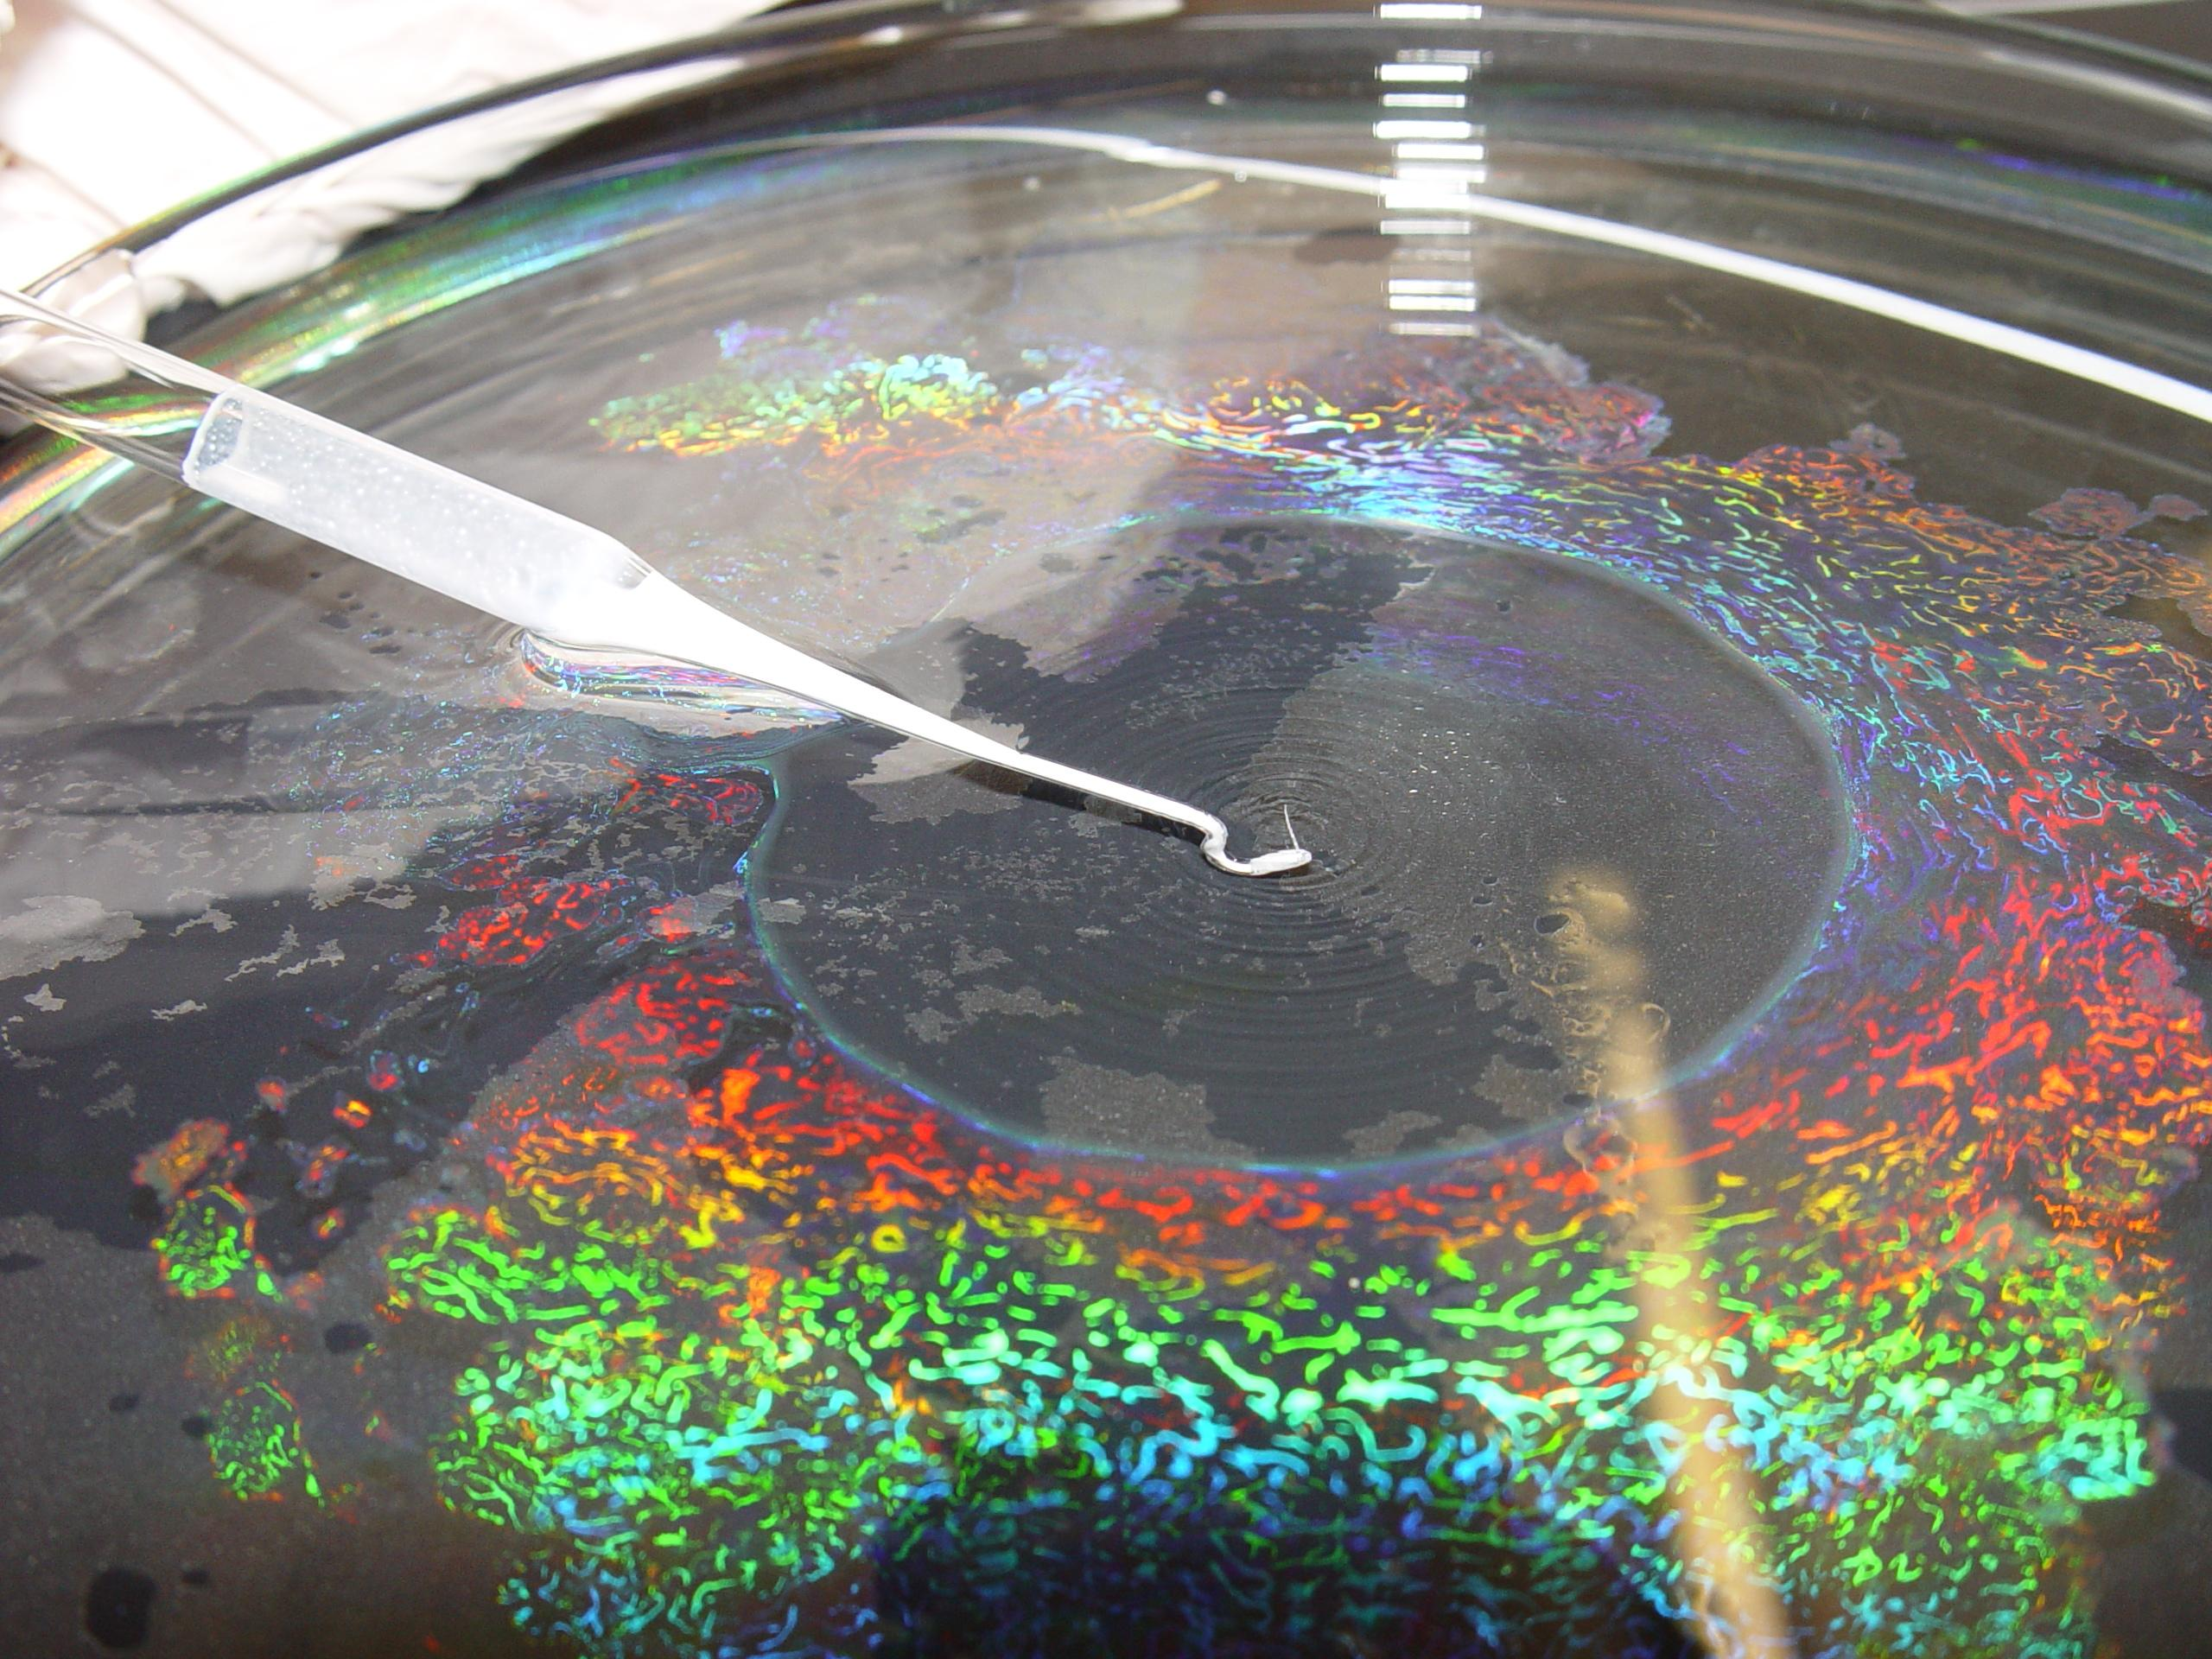
\includegraphics[width=\textwidth]{petrischale.jpg}
    \caption{Photography of (2).
        One can see the monolayer as shiny film.}
\end{subfigure}
\end{figure}
    \end{block}
\end{column}

\begin{column}{0.48\linewidth}
    \begin{block}{\circled{5} Scanning Electron Microscope Imaging (SEM)}
        \captionsetup{
    singlelinecheck=false,
    justification=justified
    }
\begin{figure}[htbp]
\begin{subfigure}{0.48\textwidth}
    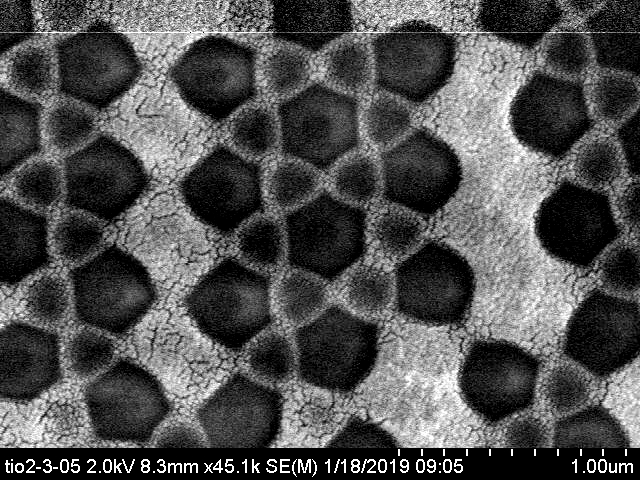
\includegraphics[width=\textwidth]{fr180-1_edited.jpg}
    \caption[justification=raggedright]{
        Full rings for \SI{180}{\second} annealing.
        }
    \label{fig:sem-fr1}
\end{subfigure}
\hfill
\begin{subfigure}{0.48\textwidth}
    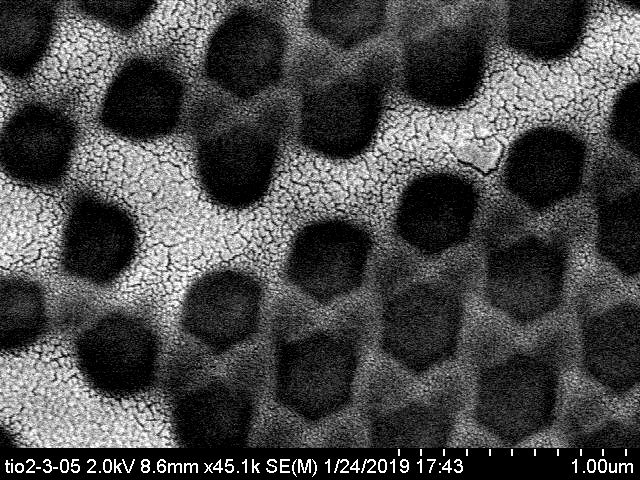
\includegraphics[width=\textwidth]{sr2180-2_edited3.jpg}
    \caption{
        Split rings for \SI{180}{\second} annealing.
    }
    \label{fig:sem-sr1}
\end{subfigure}

\begin{subfigure}{0.48\textwidth}
    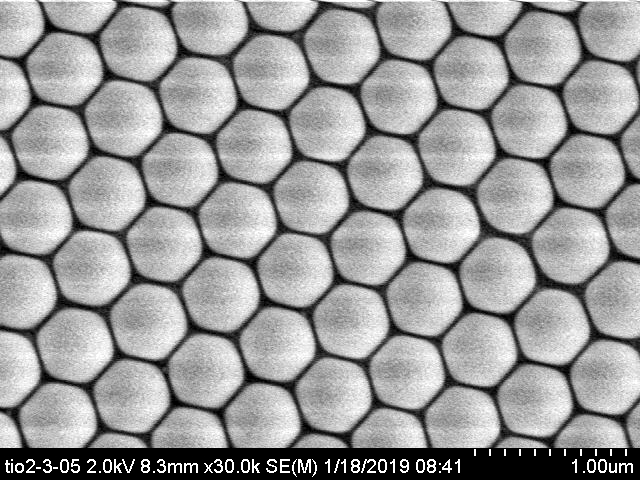
\includegraphics[width=\textwidth]{sr180-4_edited.jpg}
    \caption{
        Mask for \SI{180}{\second} annealing.
    }
    \label{fig:sem-mask}
\end{subfigure}
\hfill
\begin{subfigure}{0.48\textwidth}
    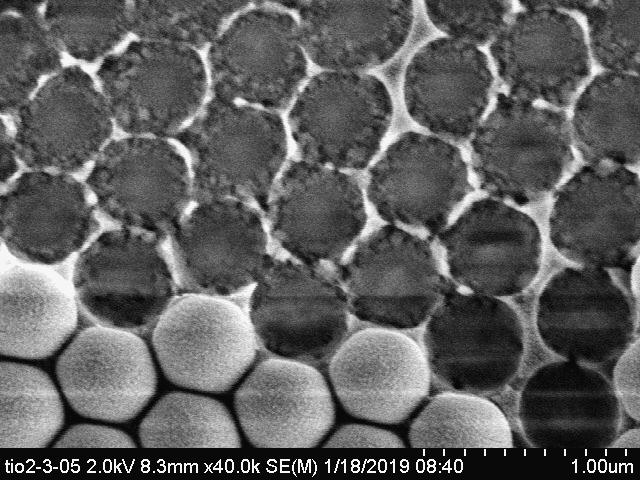
\includegraphics[width=\textwidth]{sr180-3_edited.jpg}
    \caption{
        Non sufficient annealing (\SI{180}{\second}).
    }
    \label{fig:sem-nsa}
\end{subfigure}
\end{figure}
    \end{block}

    \begin{block}{\circled{6} FTIR-Spectroscopy}
        \begin{figure}[htbp]
\begin{subfigure}{0.48\textwidth}
    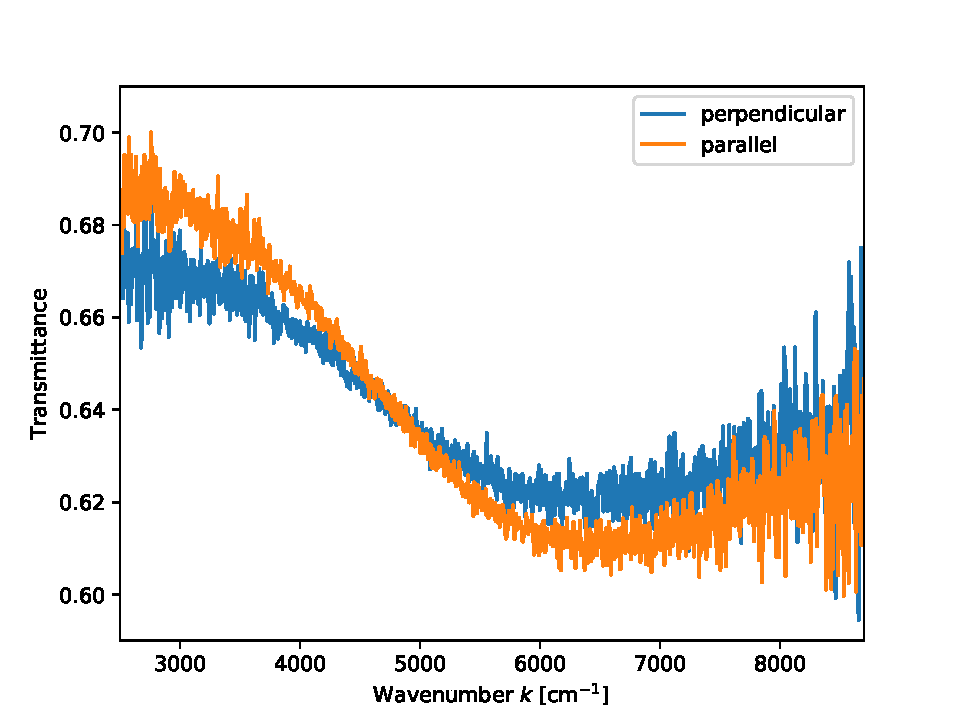
\includegraphics[width=\textwidth]{fullring.pdf}
    \caption{fullrings  }
    \label{fig:ftir_fr}
\end{subfigure}
\hfill
\begin{subfigure}{0.48\textwidth}
    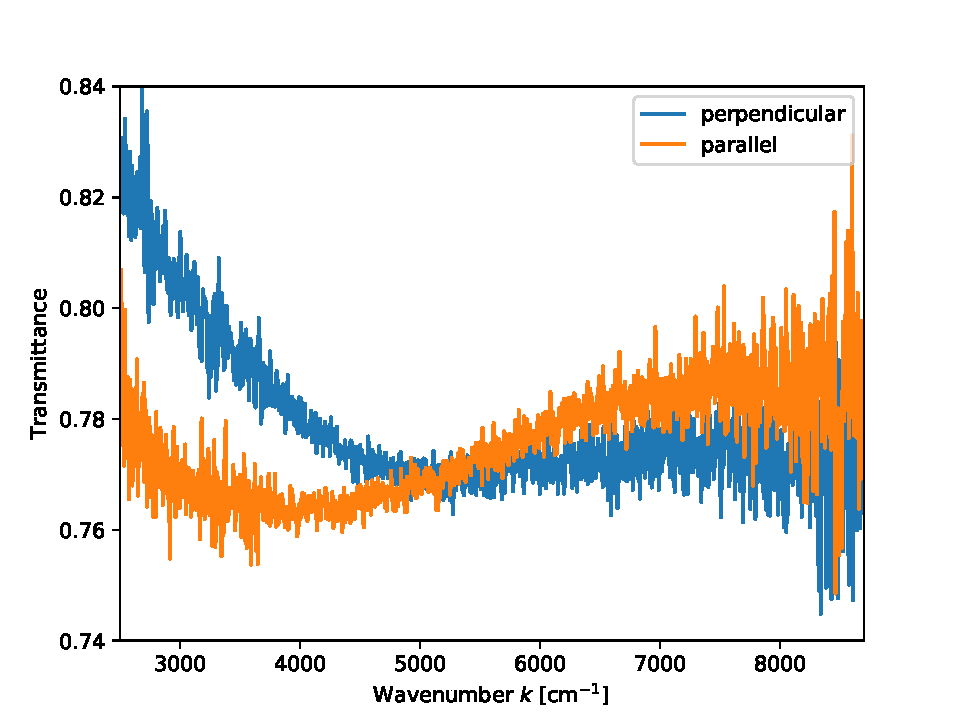
\includegraphics[width=\textwidth]{splitring.pdf}
    \caption{splitrings}
    \label{fig:ftir_sr}
\end{subfigure}
\caption{Transmittance spectra of fullrings (1) and splitrings (2) with a gap of $90^{\circ}$ between two different polarisations. }
\label{fig:ftir}
\end{figure}

\begin{itemize}
\item{There are no different plasmonen modes visible in the transmission spectra.}
\item{The difference for the SRRs between the two polarisations is too small in comparison to the theory. }
\item{The polarisation has an effect for the fullrings, which should't be the case. }
  \end{itemize}

    \end{block}

    \begin{block}{\circled{7} Conclusion}
      \begin{itemize}

\item{The split rings and the full rings overlap.} 
\item{The FTIR-spectra shows the expected behaviour, that means resonances, also when they are not so clear in comparision to the theory.}
\item{The overlapping of the rings prohibits that properties of metamaterials can occur.}
\item{Consequently one of the steps of the fabrication of the metamaterial was not succesfully, probably the annealing and wrong angles during the evaporation.}
\end{itemize}  

    \end{block}
    
    \begin{block}{Literature}
        \bibliography{mybib}{}
    \end{block}
\end{column}

\end{columns}
\end{frame}
\end{document}
